\chapter{Target Audience Questionnaire}
\label{ch:ta_questionnaire_appendix}
The questionnaire presented below was answered by 9 respondents with strong interest in football betting. 

\section{Questions}
\label{sec:ta_questions_appendix}
This questionnaire intends to collect information about the way football punters make their betting decisions (decide which team to bet on).

The questionnaire should only take around five minutes to fill in and your answers will be used to aid the development of a web application simulating the football betting experience. The future application will provide its users with all the necessary football statistics (without going too much into detail) and allow them to participate in the prediction process by making their own prediction formula. 

\textbf{Question 1}\par
\textbf{How many times a week do you bet on football or other sporting events?}
\begin{itemize}
	\item Less than once a week
	\item 1 time a week
	\item 2-3 times a week
 	\item More than 3 times a week
 \end{itemize}
 
\textbf{Question 2}\par
\textbf{How many sources of information (websites, newspapers, your favourite mobile app) do you look into before making your placing your bet?}\par
\emph{For example, if you use 2 different websites (such as BBC News and Whoscored.com), the answer is 2.}
 \begin{itemize}
 	\item None
 	\item 2-3 sources
 	\item More than 3 sources
 \end{itemize}
 
\textbf{Question 3}\par
\textbf{Please specify the sources of information that you use to support your decision.}
 \begin{itemize}
	 \item TV programmes
	 \item Sports info websites (e.g., BBC News, The Guardian)
	 \item Football info websites (e.g., whoscored.com, squawka.com)
	 \item Gambling websites (e.g., Bet365, Ladbrokes)
	 \item Betting communities or forums (e.g.,OLGB.com)
	 \item Social Networks (e.g., betting tips from football experts on Twitter)
	 \item Printed media (newspapers)
	 \item Friend's advice
	 \item Mobile apps
	 \item Specify your own: 
\end{itemize}
  
\textbf{Question 4}\par
\textbf{What main factors do you take into account before placing a bet?}\par
\emph{Choose more than one or add your own}
 \begin{itemize}
	 \item Form
	 \item League position
	 \item Result of the previous match for each team
	 \item Home/Away performance so far in the season
     \item Change of a team manager
     \item Injuries/suspensions of players
	 \item Weather
	 \item Own hunch
	 \item Specify your own: 
\end{itemize}
 
\textbf{Question 5}\par
\textbf{Do you record your betting performance?}
\begin{itemize} 
 \item Yes
 \item No
\end{itemize}

\textbf{Question 6}\par
\textbf{What statement describes you best?}
 \begin{itemize}
 	\item I only use one bookmaker to place my bets
	\item I compare the odds several bookmakers and choose the best bookmaker for each match
\end{itemize}
 
\textbf{Question 7}\par
\textbf{Would you find a web application allowing you to participate in the prediction of a match result by making up you own prediction formula useful?}
\begin{itemize}
	\item Yes
	\item No
	\item Not sure
 \end{itemize}
 
\section{Answers}
\label{sec:ta_answers_appendix}
\noindent
\begin{sidewaystable}
\begin{tabular}{
  |p{\dimexpr.1\linewidth-2\tabcolsep-1.3333\arrayrulewidth}% column 1
  |p{\dimexpr.2\linewidth-2\tabcolsep-1.3333\arrayrulewidth}% column 2
  |p{\dimexpr.2\linewidth-2\tabcolsep-1.3333\arrayrulewidth}% column 3
  |p{\dimexpr.5\linewidth-2\tabcolsep-1.3333\arrayrulewidth}|% column 4
  }
  \hline
  \centering Respondent  & \centering Question 1  & \centering Question 2 & \centering\arraybackslash Question 3   \\ \hline
  1 & 1 time a week & 2-3 sources & Sports info websites (e.g., BBC News, The Guardian), Football info websites (e.g., whoscored.com, squawka.com) \\ \hline
  2 & Less than once a week & 2-3 sources & TV programmes, Printed media (newspapers) \\ \hline
  3 & 2-3 times a week & 2-3 sources & TV programmes, Printed media (newspapers), Friends advice \\ \hline
  4 & More than 3 times a week & More than 3 sources & TV programmes, Sports info websites (e.g., BBC News, The Guardian), Gambling websites (e.g., Bet365, Ladbrokes), Betting communities or forums (e.g.,OLGB.com), Social Networks (e.g., betting tips from football experts on Twitter), Mobile apps \\ \hline
  5 & More than 3 times a week & 2-3 sources & TV programmes, Gambling websites (e.g., Bet365, Ladbrokes), Printed media (newspapers) \\ \hline
  6 & Less than once a week & 2-3 sources & Football info websites (e.g., whoscored.com, squawka.com) \\ \hline
  7 & More than 3 times a week & 2-3 sources & Football info websites (e.g., whoscored.com, squawka.com), Gambling websites (e.g., Bet365, Ladbrokes), Mobile apps \\ \hline
  8 & Less than once a week & 2-3 sources & TV programmes, Sports info websites (e.g., BBC News, The Guardian), Printed media (newspapers) \\ \hline
  9 & 2-3 times a week & 2-3 sources & Sports info websites (e.g., BBC News, The Guardian) \\ \hline
\end{tabular}
\\[10pt]
\caption{Table illustrating answers to questions 1-3 in the Target Audience Questionnaire}
\end{sidewaystable}

\noindent
\begin{sidewaystable}
\begin{tabular}{
  |p{\dimexpr.1\linewidth-2\tabcolsep-1.3333\arrayrulewidth}% column 1
  |p{\dimexpr.3\linewidth-2\tabcolsep-1.3333\arrayrulewidth}% column 2
  |p{\dimexpr.1\linewidth-2\tabcolsep-1.3333\arrayrulewidth}% column 3
  |p{\dimexpr.4\linewidth-2\tabcolsep-1.3333\arrayrulewidth}% column 4
  |p{\dimexpr.1\linewidth-2\tabcolsep-1.3333\arrayrulewidth}|% column 5
  }
  \hline
  \centering Respondent  & \centering Question 4  & \centering Question 5 &  \centering Question 6 & \centering\arraybackslash Question 7   \\ \hline
  1  & Form, League position, Result of the previous match for each team, Own hunch & No & I only one bookmaker to place my bets & Yes \\ \hline
  2 & Form, League position, Injuries/suspensions of players & No & I only use one bookmaker to place my bets & Not sure \\ \hline
  3 & Form, League position, Home/Away performance so far in the season, Own hunch & No & I compare the odds several bookmakers and choose the best bookmaker for each match & Yes \\ \hline
  4  & Form, League position, Result of the previous match for each team, Home/Away performance so far in the season, Own hunch & No & I only use one bookmaker to place my bets & Yes \\ \hline
   5 & Form, League position, Home/Away performance so far in the season, Change of a team manager & No & I compare the odds several bookmakers and choose the best bookmaker for each match & Yes \\ \hline
   6 & Form, Own hunch & No & I only use one bookmaker to place my bets & No \\ \hline
   7 & Form, Home/Away performance so far in the season, Injuries/suspensions of players & No & I only use one bookmaker to place my bets & Yes \\ \hline 
   8 & Form, League position, Result of the previous match for each team, Injuries/suspensions of players, Own hunch & No & I only use one bookmaker to place my bets & Yes \\ \hline
   9 & Form, Own hunch, Whether or not the odds appear to offer good value & No & I only use one bookmaker to place my bets & Yes \\ \hline
  \end{tabular}
 \caption{Table illustrating answers to questions 4-7 in the Target Audience Questionnaire}

\end{sidewaystable}

\chapter{Functional Requirements Review}
\label{ch:requirementsreview_appendix}

\begin{tabular}{@{}lll@{}}
        \toprule
        Requirement & Satisfied? & Comment \\
        \midrule
		\specialcell[t]{ The application will allow users to create a new account \\with the application} & Yes  & \specialcell[t]{This takes two arguments with \\ the assumption 		that the first line\\ line is longer\\ than the second.} \\ % aligned with top rule
		\specialcell[t]{ The application will allow users to sign into their accounts\\ using a web form} &  Yes & Foo bar \\ 
        \bottomrule
\end{tabular}


\chapter{User Acceptance Questionnaire}
\label{ch:ua_questionnaire_appendix}
The questionnaire presented below was answered by 7 potential end users. 

\section{Questions}
\label{sec:ua_questions_appendix}
This questionnaire intends to verify that the developed website is easy to understand and use for the potential users.

Please, complete the following steps using the application: 

\begin{enumerate}
   \item Create a new account 
   \item Login 
   \item Look through the list of matches and choose the ones you are the most interested in, then save them to dashboard
   \item Set your own prediction weights 
   \item Commit to betting on a match
\end{enumerate}

On completing the steps, please answer the following questions:

\textbf{Question 1}\par
\textbf{Which step did you find the most difficult to carry out and why?}\par
\emph{Please, provide your own answer.}
 
\textbf{Question 2}\par
\textbf{How easy was it to set up a new account?}\par
\emph{Please, rate the following question on a scale of 1 (Very easy) to 10:  (Very confusing).}
 
\textbf{Question 3}\par
\textbf{Was it easy to find and set the prediction settings?}\par
 \emph{Please, rate the following question on a scale of 1 (Very easy) to 10:  (Very confusing).}
  
\textbf{Question 4}\par
\textbf{How would you rate the overall user friendliness of the application?}\par
 \emph{Please, rate the following question on a scale of 1 (Very easy) to 10:  (Very confusing). }
 
 \textbf{Question 5}\par
\textbf{Did you find there was enough statistics to aid your decision making, and if not, what would you want to see?}\par
\emph{Please, provide your own answer.}
 
 \textbf{Question 6}\par
\textbf{What did you find was the best aspect of the application? E.g., design, navigation}\par
\emph{Please, provide your own answer.}

\textbf{Question 7}\par
\textbf{What did you find was the worst aspect of the application?}\par
\emph{Please, provide your own answer.}

\textbf{Question 8}\par
\textbf{What would you like to see in the application?}\par
\emph{Please, provide your own answer.}

\section{Answers}
\label{sec:ua_answers_appendix}

\noindent
\begin{sidewaystable}
\begin{tabular}{
  |p{\dimexpr.1\linewidth-2\tabcolsep-1.3333\arrayrulewidth}% column 1
  |p{\dimexpr.4\linewidth-2\tabcolsep-1.3333\arrayrulewidth}% column 2
  |p{\dimexpr.3\linewidth-2\tabcolsep-1.3333\arrayrulewidth}% column 3
  |p{\dimexpr.1\linewidth-2\tabcolsep-1.3333\arrayrulewidth}% column 4
  |p{\dimexpr.1\linewidth-2\tabcolsep-1.3333\arrayrulewidth}|% column 5
  }
  \hline
  \centering Respondent  & \centering Question 1  & \centering Question 2 &  \centering Question 3 & \centering\arraybackslash Question 4   \\ \hline
  1  & Probably the changing the prediction settings but even that wasn't hard really & More leagues & 10 & 8 \\ \hline
  2 & Saving matches to the dashboard, wasn't immediately apparent why I had to do that & A way to communicate with friends using the same app, maybe a separate league table for friends than just for all users & 9 & 7 \\ \hline
 3 & Committing the match, it wasn't immediately apparent that I can only commit a match previously saved in the dashboard & Maybe some news feeds & 7 & 8 \\ \hline
  4 &  Changing the prediction settings, it could have been clearer what I was supposed to do & A help menu or FAQ would be useful & 7 & 6 \\ \hline
  5 &  It was all fairly easy & More leagues, comparison betting odds from different bookies & 10 & 10 \\ \hline
  6 &  Saving matches to the dashboard, wasn't sure why I had to do that & More social interaction, link to Facebook & 8 & 7 \\ \hline
  7 &  Setting the prediction weights, wasn't sure of what to set them to so I juts left them at their default settings & A guide to how to use the app would have been nice & 10 & 7 \\ \hline

  \end{tabular}
 \caption{Table illustrating answers to questions 1-4 in the User Acceptance Questionnaire}

\end{sidewaystable}

\noindent
\begin{sidewaystable}
\begin{tabular}{
  |p{\dimexpr.1\linewidth-2\tabcolsep-1.3333\arrayrulewidth}% column 1
  |p{\dimexpr.1\linewidth-2\tabcolsep-1.3333\arrayrulewidth}% column 2
  |p{\dimexpr.3\linewidth-2\tabcolsep-1.3333\arrayrulewidth}% column 3
  |p{\dimexpr.3\linewidth-2\tabcolsep-1.3333\arrayrulewidth}% column 4
  |p{\dimexpr.2\linewidth-2\tabcolsep-1.3333\arrayrulewidth}|% column 5
  }
  \hline
  \centering Respondent  & \centering Question 5  & \centering Question 6 &  \centering Question 7 & \centering\arraybackslash Question 8   \\ \hline
  1  & 8 & The layout was easy on the eye and simple enough to find your way about & Not enough football leagues represented & Yes \\ \hline
  2 & 5 & The design was simple but nice to look at & The dashboard seems a but pointless & Yes \\ \hline
  3 & 8 & The prediction feature was great, especially because I could change it myself & The design was a little boring & Yes \\ \hline
  4 & 5 & The way the stats and matches were presented, very clear & The way to change the prediction settings could have been explained better & Yes \\ \hline
  5 &  10 & It was very self explanatory how it all worked together & Lack of football leagues to use & No, betting odds \\ \hline
  6 &  7 & I liked the design & The dashboard wasn't very useful & Yes \\ \hline
  7 &  5 &  Navigating from page to page was easy & I was confused about the prediction settings & Yes \\ \hline

  \end{tabular}
 \caption{Table illustrating answers to questions 5-7 in the User Acceptance Questionnaire}

\end{sidewaystable}
 
\chapter{Installation Instructions}
\label{ch:install_appendix}
The code can be checked out using git by executing the following command in the terminal:

\noindent See the following command :
\begin{lstlisting}[language=bash]
  $ git clone git@github.com:marinamarina/sure-thing.git
\end{lstlisting}

Installation instructions are found at the following url:

\url{https://www.github.com:marinamarina/sure-thing/blob/master/README.md}.


If any issues arise regarding installation of any part of the system, do not hesitate to contact me at 1014481@rgu.ac.uk

\chapter{Credits}
\label{ch:credits_appendix}
Some the application's code was taken from the GitHub repository accompanying the book by Miguel Grindberg "Flask Web Development" \citep{book:Grindberg2014FlaskWebDevelopment}. Below are listed the components of the system that rely on this code to some extent:

\begin{itemize}
	\item user authentication, account verification
	\item basic test suite
	\item user authentication test suite
\end{itemize}

Some of the handy decorator functions used in the Python code were taken from Flask documentation \citep{documentation:Flask}, section "View Decorators".

\chapter{Project Management}
\label{ch:pm_appendix}
The project was not developed following a single software development methodology. Different techniques from various methodologies were used for the project. Some of the planning was made beforehand in the traditional, Waterfall approach fashion, such as researching the project background, defining application requirements, sketching the application wireframes, etc. On the other hand, some of the design techniques were adopted from the Agile methodology, namely user journeys. 

The project implementation phase was carried out in an iterative manner. For defining the project requirements, the application functionality was divided into clearly defined units (so called "high-level features" introduced in the chapter "Requirements Analysis" \ref{ch:requirementanalysis}), each associated with an implementation iteration. Excel sheets were used for defining the set of tasks for each iteration. GitHub issue tracker was also used as a supporting productivity tool for this project. Code related tasks were recorded as "issues" for the project GitHub repository. In general, the GitHub issue tracker was a very efficient tool for keeping the project organised. 

\chapter{Presentation Slides}
\label{ch:slides_appendix}
These are the slides used for the project presentation.

\begin{figure}[ht!]
\centering
	\fbox{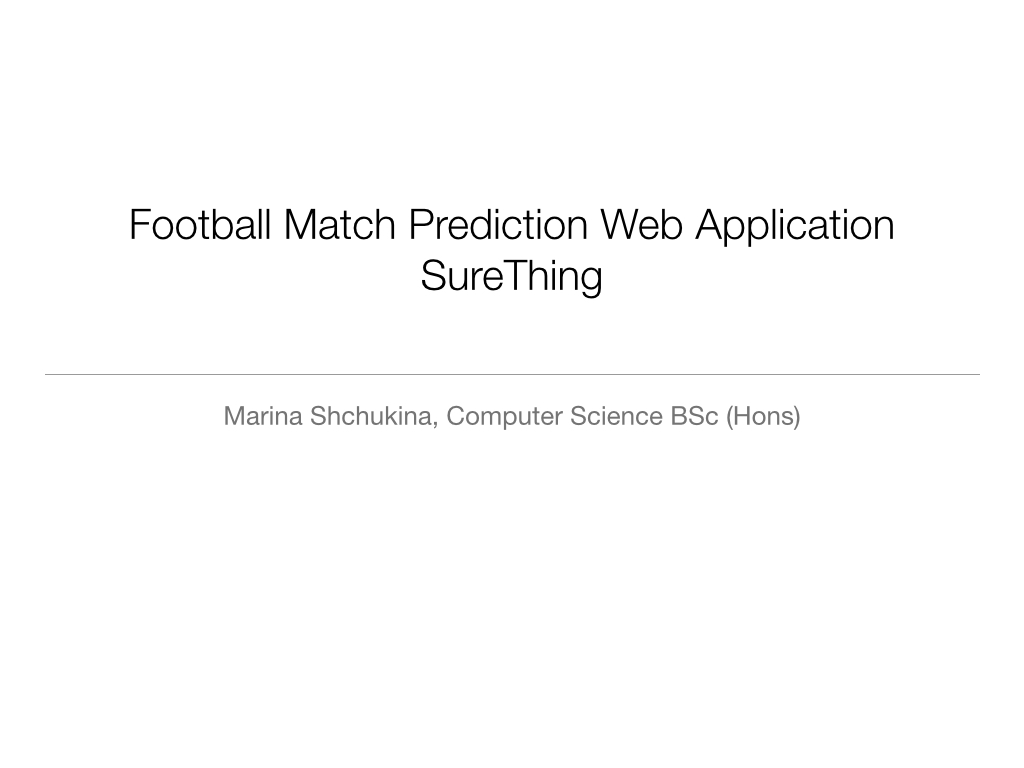
\includegraphics[width=0.7\columnwidth]{appendix/images/slides001.jpg}}
	\caption{Slide 1 of the presentation \label{slide1}}
\end{figure}

\begin{figure}[ht!]
\centering
	\fbox{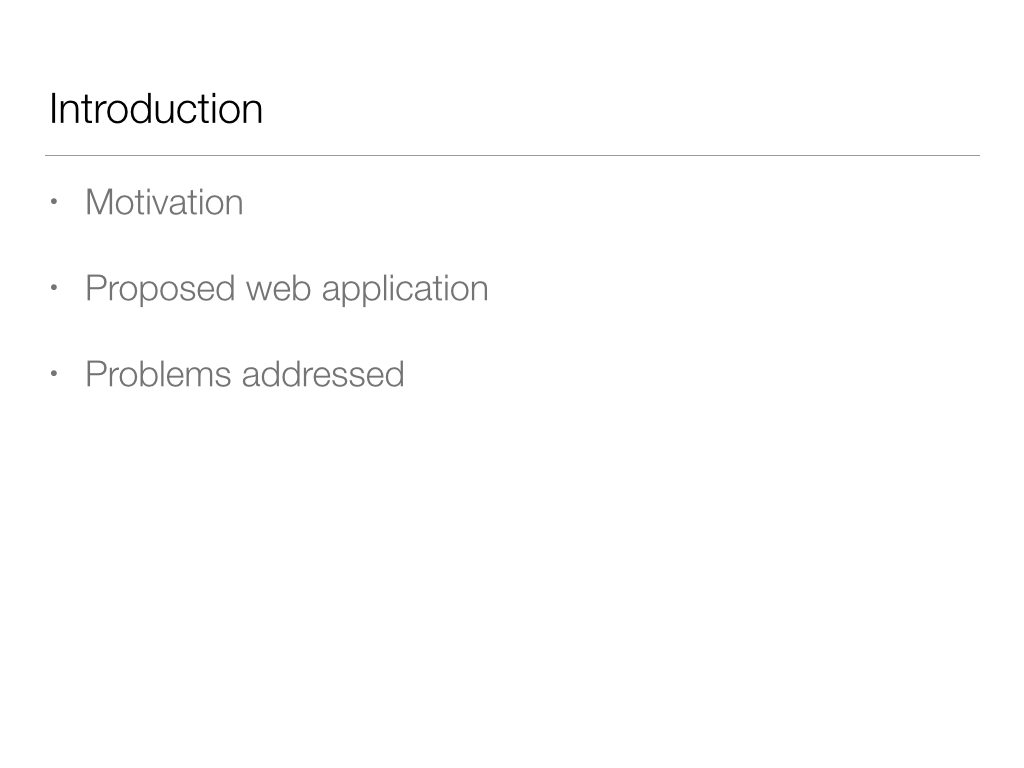
\includegraphics[width=0.7\columnwidth]{appendix/images/slides002.jpg}}
	\caption{Slide 2 of the presentation \label{slide2}}
\end{figure}

\begin{figure}[ht!]
\centering
	\fbox{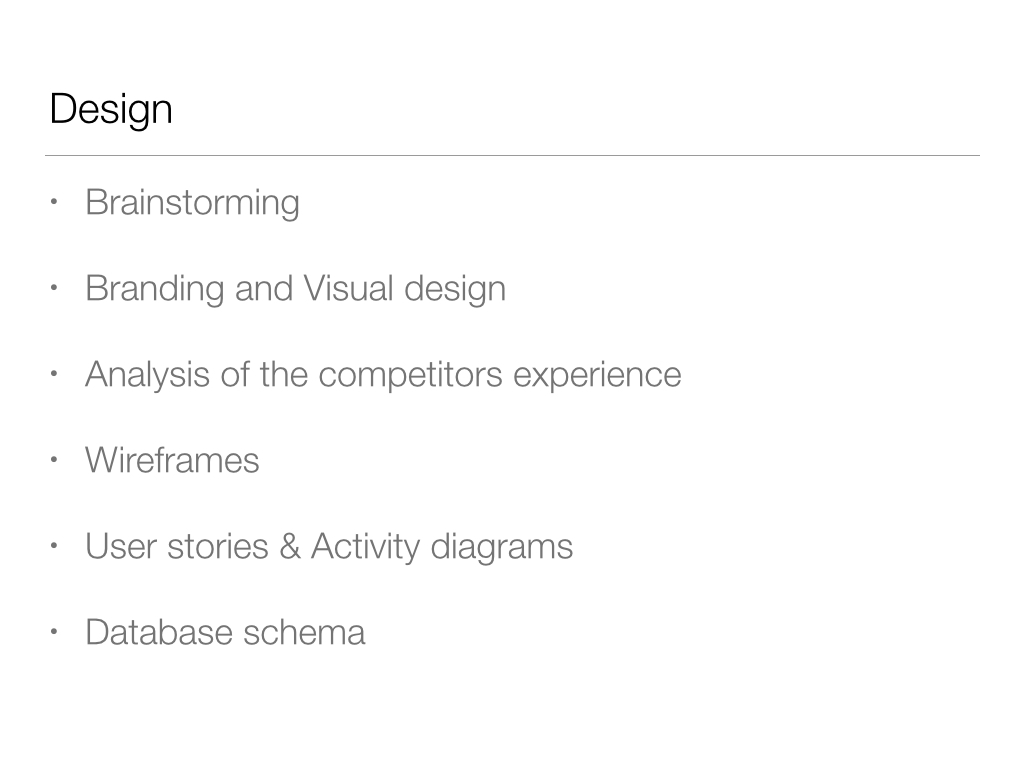
\includegraphics[width=0.7\columnwidth]{appendix/images/slides003.jpg}}
	\caption{Slide 3 of the presentation \label{slide3}}
\end{figure}

\begin{figure}[ht!]
\centering
	\fbox{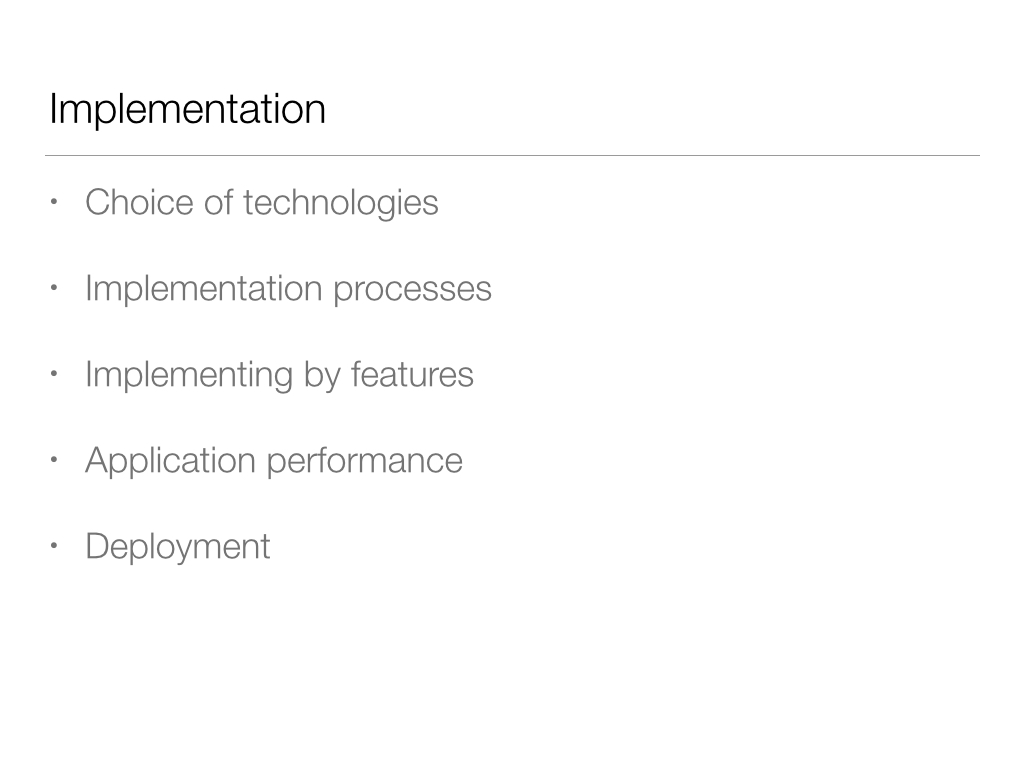
\includegraphics[width=0.7\columnwidth]{appendix/images/slides004.jpg}}
	\caption{Slide 4 of the presentation \label{slide4}}
\end{figure}

\begin{figure}[ht!]
\centering
	\fbox{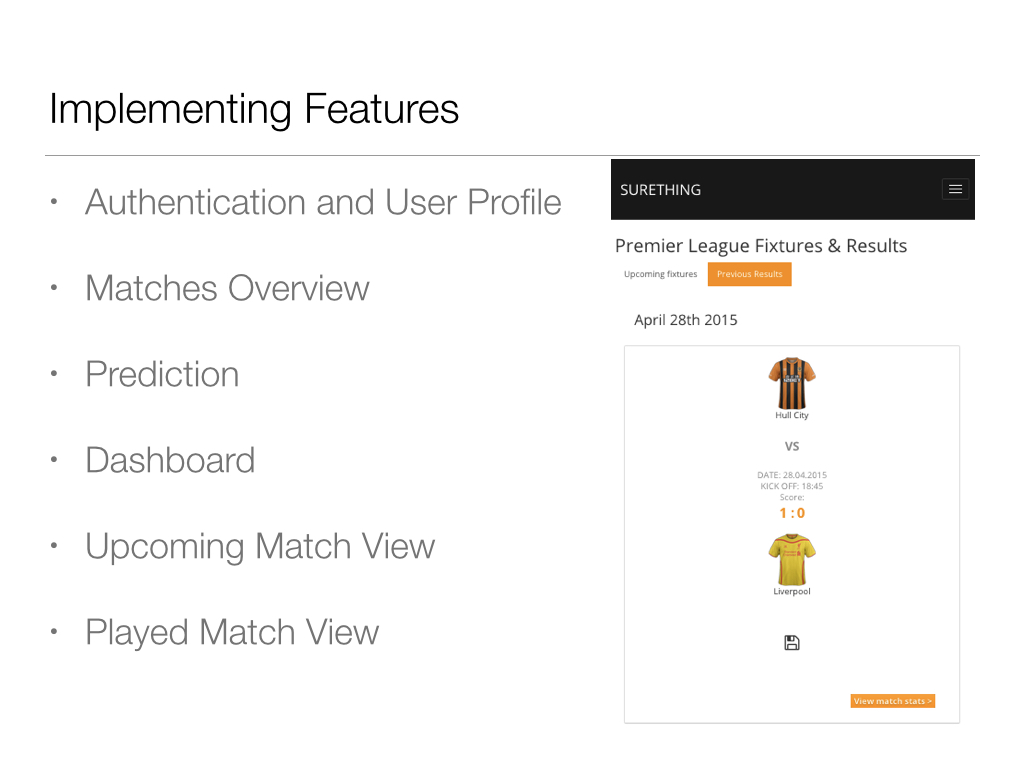
\includegraphics[width=0.7\columnwidth]{appendix/images/slides005.jpg}}
	\caption{Slide 5 of the presentation \label{slide5}}
\end{figure}

\begin{figure}[ht!]
\centering
	\fbox{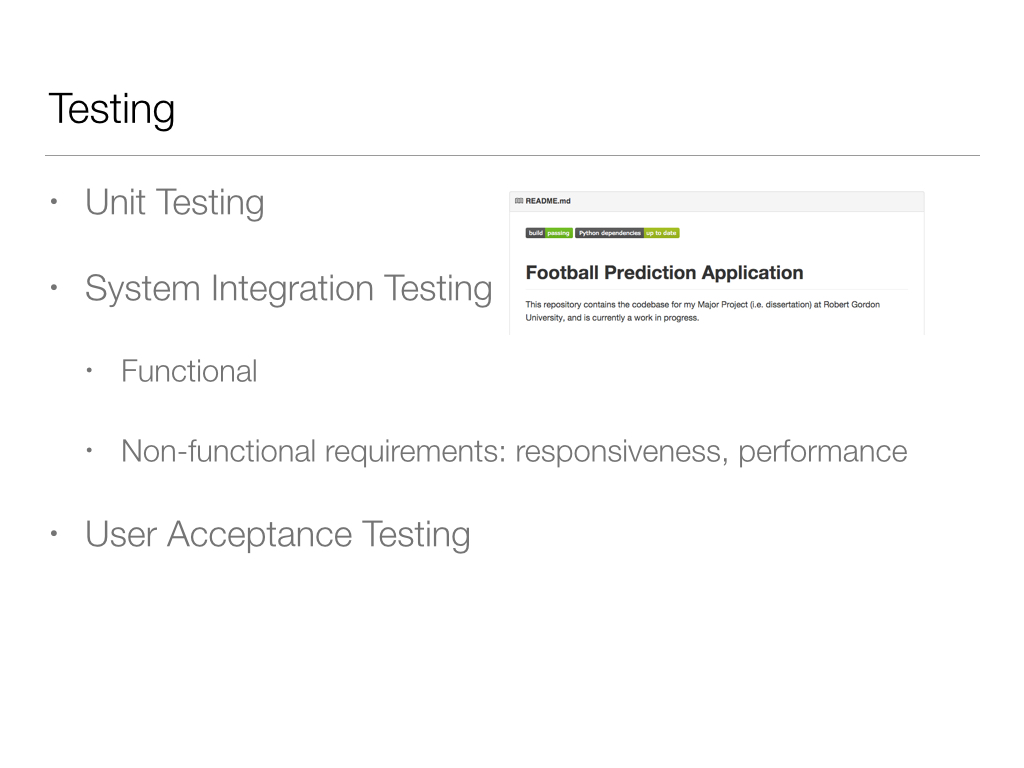
\includegraphics[width=0.7\columnwidth]{appendix/images/slides006.jpg}}
	\caption{Slide 6 of the presentation \label{slide6}}
\end{figure}

\begin{figure}[ht!]
\centering
	\fbox{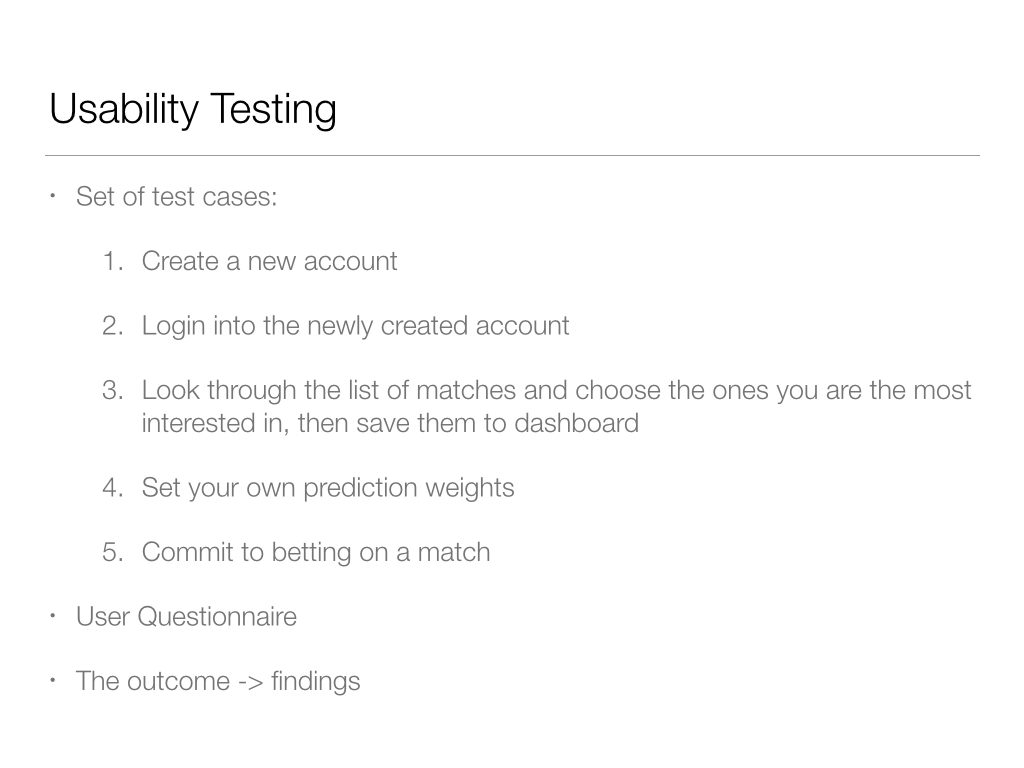
\includegraphics[width=0.7\columnwidth]{appendix/images/slides007.jpg}}
	\caption{Slide 7 of the presentation \label{slide7}}
\end{figure}

\begin{figure}[ht!]
\centering
	\fbox{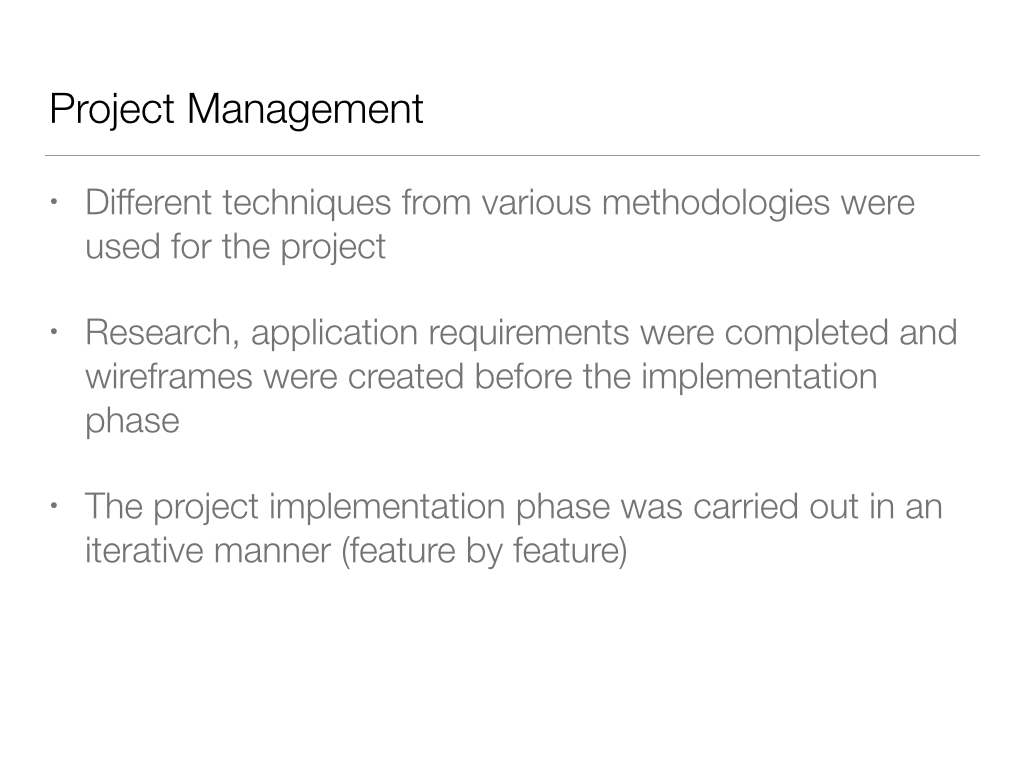
\includegraphics[width=0.7\columnwidth]{appendix/images/slides008.jpg}}
	\caption{Slide 8 of the presentation \label{slide8}}
\end{figure}







